%%%%%%%%%%%%%%%%%%%%%%%%%%%%%%%%%%%%%%%%%%%%%%%%%%%%%%%%%%%%%%%%%%%%%
% 
% Certains éléments de ce documents ont été repris des templates suivants :
%
%Original Source: http://www.howtotex.com
% https://tex.stackexchange.com/a/86310/10898
%http://cacr.uwaterloo.ca/~dstinson/papers/pseudocode.pdf
%
%%%%%%%%%%%%%%%%%%%%%%%%%%%%%%%%%%%%%%%%%%%%%%%%%%%%%%%%%%%%%%%%%%%%%%

\documentclass{article}
\usepackage[a4paper]{geometry}
\usepackage[myheadings]{fullpage}
\usepackage{fancyhdr}
\usepackage{lastpage}
\usepackage[T1]{fontenc}
\usepackage[utf8]{inputenc}
\usepackage{fourier}
\usepackage[protrusion=true, expansion=true]{microtype}
\usepackage[french]{babel}
\usepackage{graphicx, wrapfig, subcaption, setspace, booktabs}
\usepackage[font=small, labelfont=bf]{caption}
\usepackage{sectsty}
\usepackage{url, lipsum}
\usepackage{amsmath}
\usepackage{tikz}
\usepackage{epigraph}
\usepackage{verbatim}
\usepackage{fancybox}
\usepackage{pseudocode}
\usepackage{epsfig}
\usepackage{float}
\usepackage{titlesec}
\usepackage{url}
\usepackage{longtable}
\usepackage{colortbl}
\usepackage{pdfpages}
\usepackage{subscript}

\expandafter\def\expandafter\UrlBreaks\expandafter{\UrlBreaks
  \do\*\do\-\do\~\do\'\do\"\do\_} %URL breaklines


\newcommand{\ptitre}[1]{\vspace{0.3 cm}• \textbf{#1 :}} % \ptitre{titre}
\renewcommand\epigraphflush{flushright}
\renewcommand\epigraphsize{\normalsize}
\setlength\epigraphwidth{0.7\textwidth}

\definecolor{titlepagecolor}{rgb}{1.0,1.0,0.6}

\newcommand\titlepagedecoration{%
\begin{tikzpicture}[remember picture,overlay,shorten >= -10pt]

\coordinate (aux1) at ([yshift=-15pt]current page.north east);
\coordinate (aux2) at ([yshift=-410pt]current page.north east);
\coordinate (aux3) at ([xshift=-4.5cm]current page.north east);
\coordinate (aux4) at ([yshift=-150pt]current page.north east);
\coordinate (aux5) at ([yshift=-550pt]current page.north east);


\begin{scope}[titlepagecolor!40,line width=12pt,rounded corners=12pt]
\draw
  (aux1) -- coordinate (a)
  ++(225:5) --
  ++(-45:5.1) coordinate (b);
\draw[shorten <= -10pt]
  (aux3) --
  (a) --
  (aux1);
\draw[opacity=0.6,titlepagecolor,shorten <= -10pt]
  (b) --
  ++(225:2.2) --
  ++(-45:2.2);
\end{scope}
\draw[titlepagecolor,line width=8pt,rounded corners=8pt,shorten <= -10pt]
  (aux4) --
  ++(225:0.8) --
  ++(-45:0.8);
\begin{scope}[titlepagecolor!70,line width=6pt,rounded corners=8pt]
\draw[shorten <= -10pt]
  (aux2) --
  ++(225:3) coordinate[pos=0.45] (c) --
  ++(-45:3.1);
\draw
  (aux2) --
  (c) --
  ++(135:2.5) --
  ++(45:2.5) --
  ++(-45:2.5) coordinate[pos=0.3] (d);   
\draw 
  (d) -- +(45:1);
\end{scope}
\end{tikzpicture}%
}

\newcommand{\HRule}[1]{\rule{\linewidth}{#1}}
\onehalfspacing
\setcounter{tocdepth}{5}
\setcounter{secnumdepth}{5}

%-------------------------------------------------------------------------------
% HEADER & FOOTER
%-------------------------------------------------------------------------------
\pagestyle{fancy}
\fancyhf{}
\setlength\headheight{15pt}
\fancyhead[L]{DUBOURDIEU, JOLY, MARLIER}
\fancyhead[R]{Le Graal de l'intégration}
\fancyfoot[R]{\thepage\ / \pageref{LastPage}}
%-------------------------------------------------------------------------------
% TITLE PAGE
%-------------------------------------------------------------------------------

 
\title{ \normalsize \textsc{Projet C 2017-2018}
		\\ [2.0cm]
		\HRule{0.5pt}
		\\ [1.0cm]
		\LARGE \textbf{\uppercase{Le Graal de l'intégration}}
    	\\ [1.0cm]
		\HRule{0.5pt} \\
		\LARGE \textsc{Partie 1 : Gestion de projet}
		\HRule{2pt} 
		\\ [0.5cm]
		\normalsize \vspace*{3\baselineskip}
		}

\date{}



\author{DUBOURDIEU Lucas \\ 
	    JOLY Clément \\
		MARLIER Romain }

\begin{document}

\maketitle
\begin{figure}[b]
    \centering
    
\includegraphics[scale=0.32]{logo.png}
\end{figure}
\thispagestyle{empty}
\titlepagedecoration

\newpage

\tableofcontents
\newpage
%-------------------------------------------------------------------------------
% Section title formatting
\sectionfont{\scshape}
%-------------------------------------------------------------------------------

%-------------------------------------------------------------------------------
% Body
%-------------------------------------------------------------------------------
\section{Introduction}

Le projet \textit{Le Graal de l'intégration} a été donné aux élèves de la promotion 2020 de TELECOM Nancy. Ce projet a pour but de \textit{nous familiariser avec la programmation modulaire, et l’usage du langage C. Il doit également nous permettre de nous familiariser avec les structures de données (implantation, utilisation)}. \\

L'objectif du programme a ainsi été défini : \\

\textit{L’objectif de ce projet est de concevoir, développer et tester un système de recommandation de films, similaire à ceux qui peuvent être proposés sur les téléviseurs intelligents (smart TVs). Grâce à ce système, l’utilisateur indique une liste des films qu’il a déjà regardés, et obtient en retour une liste de films recommandés/suggérés à partir d’une analyse de ses préférences [...] au travers d’une interface graphique.} \\

\section{Étude du projet}

\subsection{Présentation}


En s'appuyant sur la présentation du sujet ci-dessus, nous avons défini le projet comme suit :

\begin{figure}[H]
    \centering
    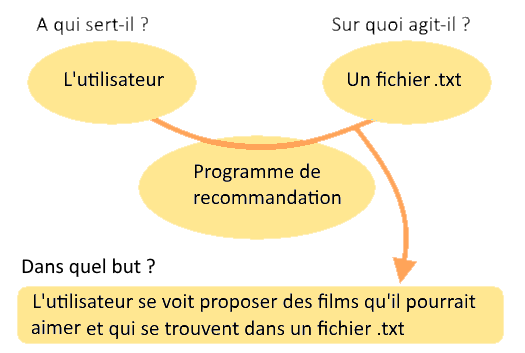
\includegraphics[scale=0.5]{GDP/bete.png}
    \caption{\label{bete} Diagramme de la bête à corne}
\end{figure}

Afin de répondre à toutes les attentes, le programme de recommandation devra intéragir avec plusieurs éléments extérieurs et donc répondre à certaines fonctions de contraintes.

\begin{figure}[H]
    \centering
    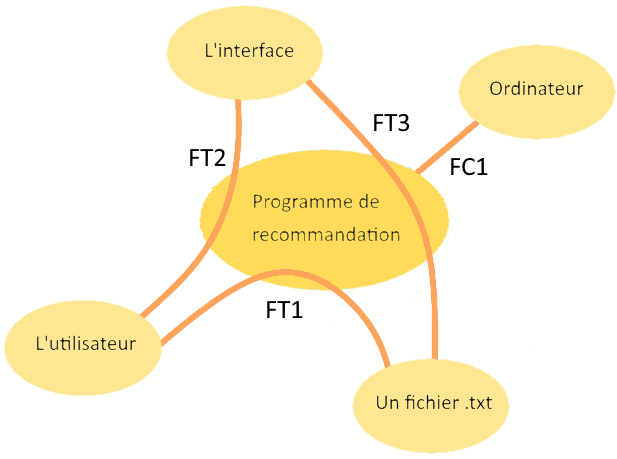
\includegraphics[scale=0.5]{GDP/pieuvre.png}
    \caption{\label{pieuvre} Diagramme pieuvre}
\end{figure}

\begin{longtable}[c]{|c|c|}
\hline
\textbf{Fonction de contrainte} & Ne pas demander trop de ressources à l'utilisateur             \\ \hline
\endfirsthead

\endhead

\textbf{Fonction technique 1}   & L'utilisateur peut choisir un film appartenant au fichier .txt \\ \hline
\textbf{Fonction technique 2}   & L'utilisateur peut utiliser facilement l'interface             \\ \hline
\textbf{Fonction technique 3}   & L'interface présente les films du fichier .txt                 \\ \hline
\caption{Tableau récapitulatif des fonctions des fonctions de contraintes et techniques}
\label{tab1}\\
\end{longtable}

Dans le but de répondre au mieux à la résolution de ces fonctions techniques, nous avons mis en place un diagramme \textbf{FAST} (Functional Analysis System Technique) du projet. Le projet est ainsi découpé en plusieurs étapes, chacune complétée par une solution technique réalisable.


\begin{figure}[H]
    \centering
    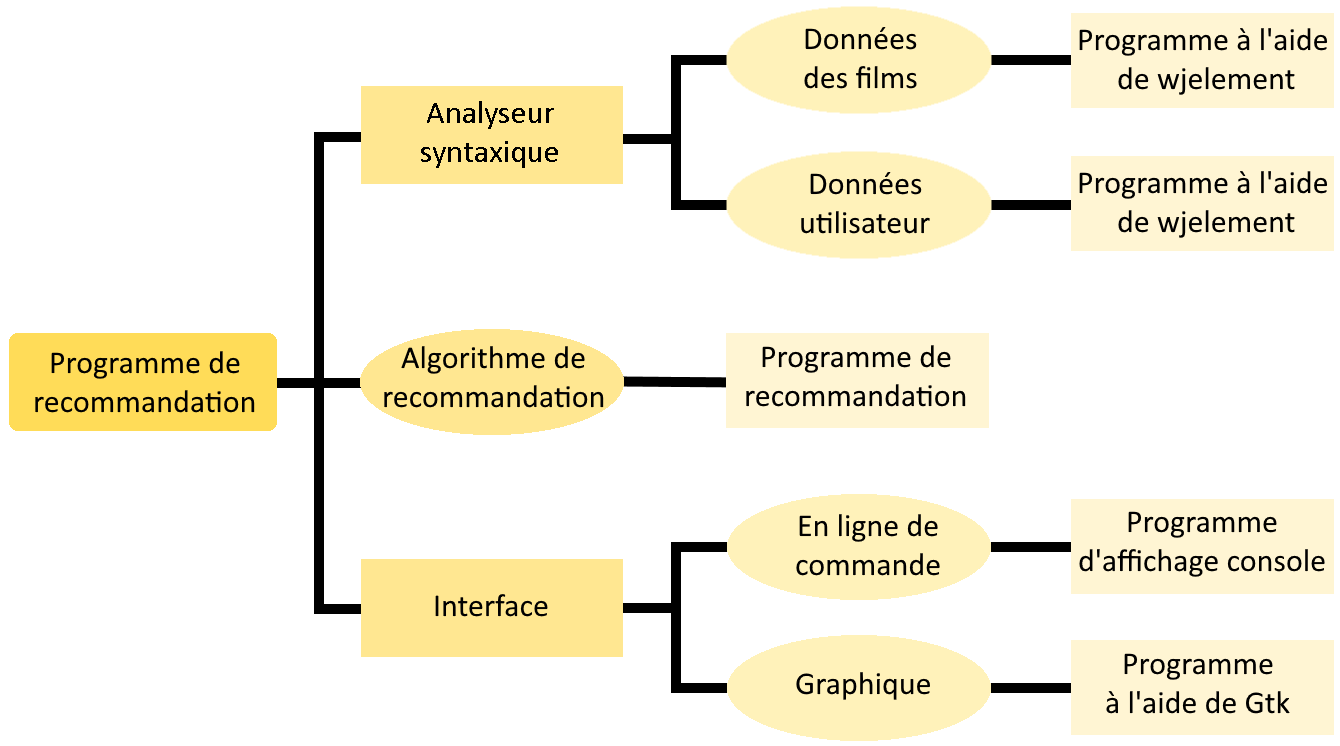
\includegraphics[scale=0.4]{GDP/fast.png}
    \caption{\label{fast} Diagramme FAST}
\end{figure}


\subsection{Faisabilité}

Le projet ainsi défini, il convient de vérifier si sa réalisation est possible. Une étude \textbf{SMART} (Spécifique / Mesurable / Accepté / Réaliste / Temporel) portant sur l'ensemble du sujet à donc été réalisée.

\begin{figure}[H]
    \centering
    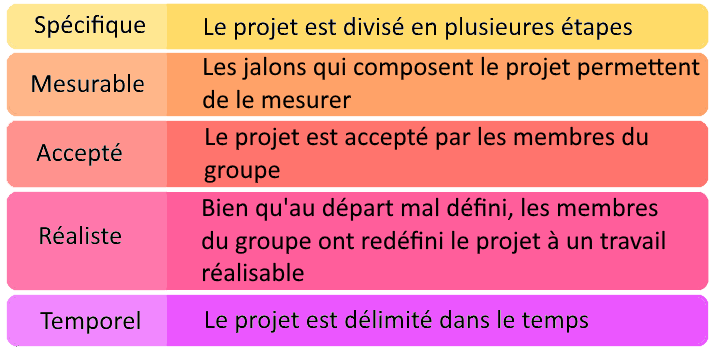
\includegraphics[scale=0.5]{GDP/smart.png}
    \caption{\label{smart} Méthode SMART}
\end{figure}

Le projet répond aux attentes d'un projet traditionnel, il est donc légitime.


\subsection{Mise en place}

Le projet a été divisé en plusieurs étapes. Ces étapes ont ensuite été priorisées et délimitées dans le temps afin d'optimiser au mieux la réalisation du projet. Un diagramme \textbf{Gantt} a donc vu le jour afin d'expliciter les étapes du projet ainsi que son jalonnement.

\begin{figure}[H]
    \centering
   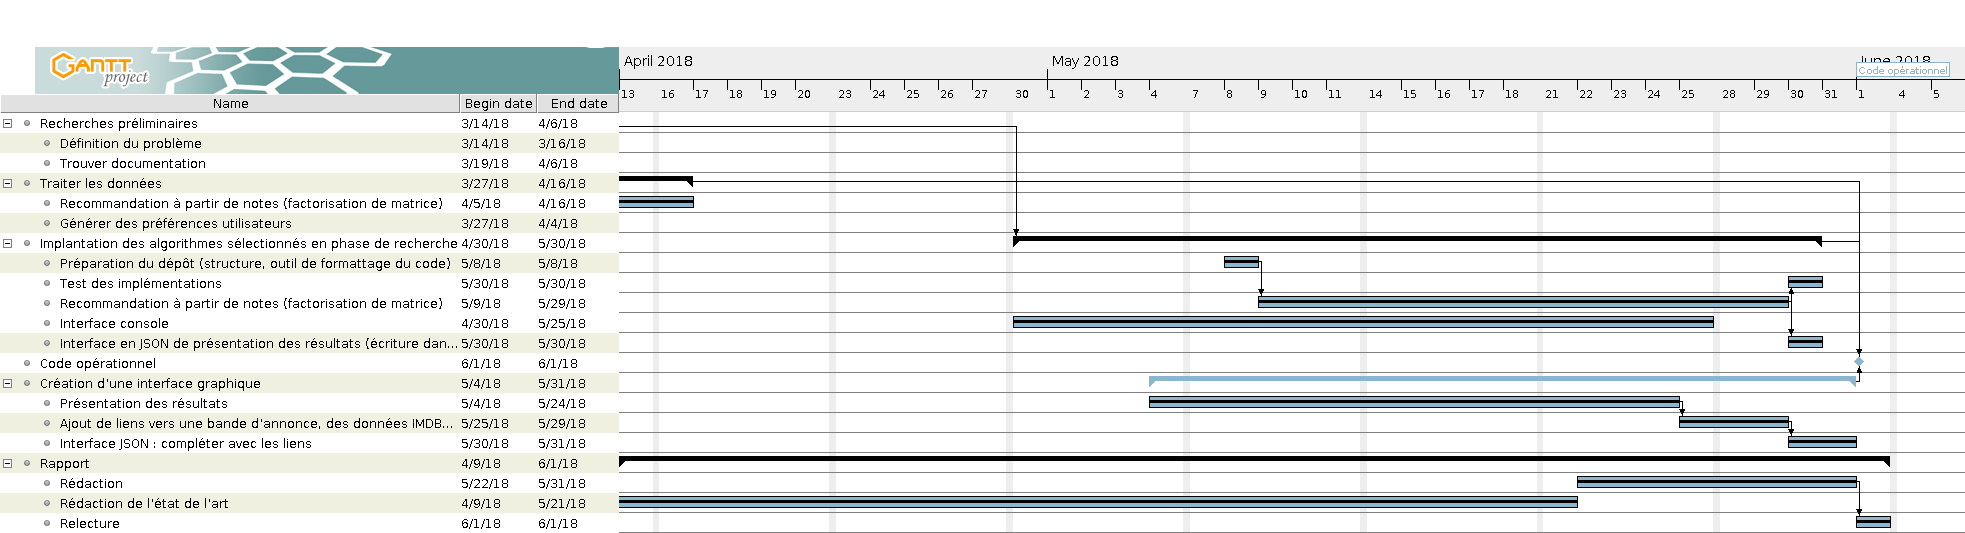
\includegraphics[scale=0.23]{GDP/gantt.png}
    \caption{\label{gant} Diagramme Gantt}
\end{figure}

\section{Organisation du groupe}
\subsection{Les prémices de l'organisation}

Les membres de l'équipe projet ont tout d'abord décidé de se répartir les rôles afin de structurer l'équipe. Le rôle de chef de projet a été confié à Lucas DUBOURDIEU. Il aura pour rôle d'animer les réunions et de déposer le rapport final sur la plate-forme Arche dédiée au rendu du projet. Afin de répartir le travail le rôle de secrétaire sera attribué à tour de rôle aux différents membres du trinôme. La répartition des rôles peut être représentée ainsi :

\begin{longtable}[c]{|c|c|}

\hline
\rowcolor[HTML]{F2D396} 
\textbf{Chef de projet/secrétaire} & DUBOURDIEU Lucas \\ \hline
\endfirsthead
%
\endhead
%
\textbf{Secrétaire} & JOLY Clément     \\ \hline
\rowcolor[HTML]{F2D396} 
\textbf{Secrétaire}  & MARLIER Romain   \\ \hline
\caption{Tableau de répartition des rôles}
\label{tab2}\\
\end{longtable}

Le projet ayant été divisé en plusieurs tâches, celles-ci ont été attribuées aux différents membres du groupe. Un responsable a été nommé pour chaque tâche. Néanmoins, les membres du groupe aident an amont et en aval la réalisation des tâches dont ils ne sont pas responsables. Les questionnements ainsi que les différentes décisions sont le fruit d'un travail d'équipe qui permet ainsi à chaque responsable d'être ni démotivé ni bloqué dans son travail. Une matrice \textbf{RACI} permet d'expliciter l'attribution de chaque lot de travail.

\begin{longtable}[c]{|
>{\columncolor[HTML]{FFFFC7}}c |c|c|c|}
\hline
\cellcolor[HTML]{F2D396}\textbf{Lot de travail} & \cellcolor[HTML]{F2D396}\textbf{Lucas DUBOURDIEU} & \cellcolor[HTML]{F2D396}\textbf{Clément JOLY} & \cellcolor[HTML]{F2D396}\textbf{Romain MARLIER} \\ \hline
\endfirsthead
%
\endhead
%
\textbf{État de l'art} & RA & CI & CI \\ \hline
\textbf{Outils de gestion de projet} & RA  & CI  & CI \\ \hline
\textbf{Exploitation de fichiers JSON}  & CI & CI & RA   \\ \hline
\textbf{Programme de recommandation} & CI & RA  & CI \\ \hline
\textbf{Interface en ligne de commande}  & CI  & CI  & RA  \\ \hline
\textbf{Interface graphique} & RA & CI  & CI \\ \hline
\caption{Matrice RACI}
\label{tab3}\\
\end{longtable}

\begin{longtable}[c]{ll}
R : Responsable & A : Acteur, exécutant de la tâche \\
\endfirsthead
\endhead
C :Consulté avant la réalisation de la tâche & I : Informé de la réalisation de la tâche
\end{longtable}


\subsection{Accréditation du travail}

Le projet correctement défini et l'équipe de projet formée, nous avons réaliser une matrice \textbf{SWOT} (Strenghts Weaknesses Opportunities Threats) afin d'évaluer les forces et les menaces, qu'elles soit internes ou externes au projet. En accord avec la définition d'une matrice SWOT, les cases Strenghts et Weaknesses correspondent à un diagnostic internes tandis que les cases Opportunities et Threats caractérisent le diagnostic externe.

\begin{figure}[H]
    \centering
    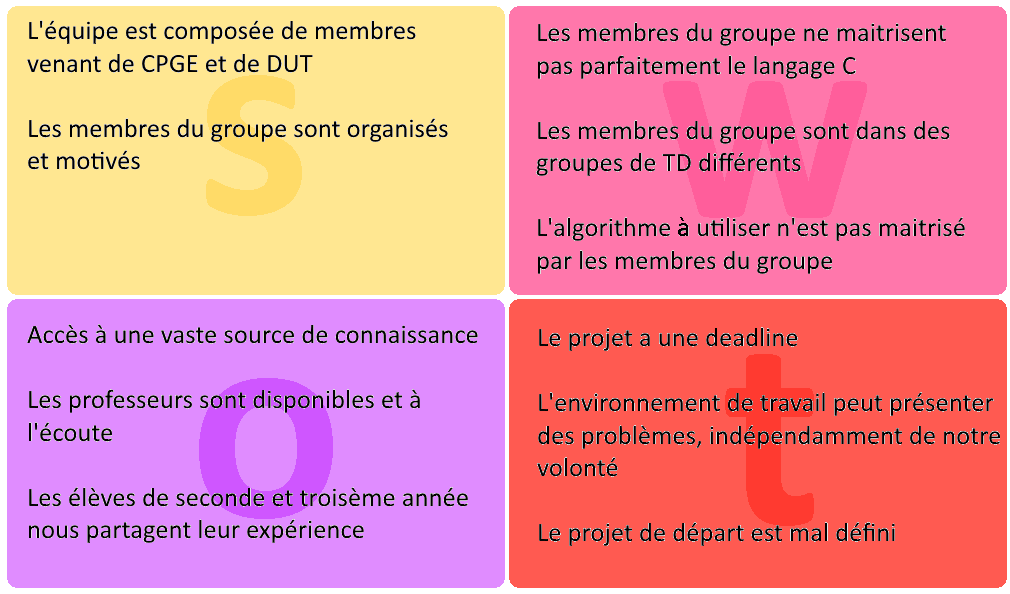
\includegraphics[scale=0.5]{GDP/swot.png}
    \caption{\label{swot} Matrice SWOT}
\end{figure}

Afin de jalonner le projet et d'éviter un sentiment de démotivation auprès des membres du groupe, des réunions hebdomadaires ont été effectuées. Ces réunions permettaient de partager le travail de chacun et de fixer de nouveaux objectifs.


\section{Bilan}
\subsection{Fiche de définition du projet}

La \textbf{fiche est bilan} est un tableau qui permet de récapituler les informations précédentes. La réalisation de cette fiche annonce le lancement du projet.


\begin{longtable}[c]{|
>{\columncolor[HTML]{F2D396}}l |l|}
\hline
\textbf{Les enjeux}                                                                      & \begin{tabular}[c]{@{}l@{}}Le projet s'adresse aux élèves de la promotion 2020 de TELECOM Nancy.\\ Il permettra la validation du module C.\end{tabular}                                                                                                                                                                                                                                                                          \\ \hline
\endfirsthead
%
\endhead
%
\textbf{Le contexte}                                                                     & \begin{tabular}[c]{@{}l@{}}Afin de mettre en avant leur contenu, qu'il soit multimédia ou matériel, de\\ plus en plus de sites internet ou d'application utilisent des systèmes de\\ recommandation. L'efficacité et l'efficience de ces systèmes sont des enjeux\\ majeurs pour la pérennité de l'entreprise.\\ \\ Le projet a été étudié (matrice SWOT), divisé (diagramme FAST) et est\\ délimité dans le temps.\end{tabular} \\ \hline
\textbf{\begin{tabular}[c]{@{}l@{}}Les résultats attendus,\\ les livrables\end{tabular}} & \begin{tabular}[c]{@{}l@{}}L'équipe projet livrera un rapport final avant le 01/06/2018. Ce rapport\\ présentera les outils de gestion de projet mis en place, l'état de l'art ainsi\\ que le travail accompli.\end{tabular}                                                                                                                                                                                                     \\ \hline
\textbf{Les risques}                                                                     & \begin{tabular}[c]{@{}l@{}}Le facteur humain est un risque majeur à la réalisation de tout projet.\\ Le projet et délimité dans le temps, cette limite est une menace à\\ l'aboutissement du projet.\\ Il ne faut pas négliger les risques exterieurs tel que l'environnement de\\ travail,...\end{tabular}                                                                                                                      \\ \hline
\textbf{\begin{tabular}[c]{@{}l@{}}Le budget : les moyens \\ et ressources\end{tabular}} & \begin{tabular}[c]{@{}l@{}}Le projet sera réalisé par trois élèves ingénieurs de la promotion 2020 de\\ TELECOM Nancy.\\ \\ Les ordinateurs de TELECOM Nancy ainsi que leurs ordinateurs\\ personnels sont à leur disposition.\end{tabular}                                                                                                                                                                                      \\ \hline
\textbf{Les acteurs}                                                                     & \begin{tabular}[c]{@{}l@{}}Ayant pour chef de projet Lucas DUBOURDIEU, l'équipe est complétée\\ par Clément JOLY et Romain MARLIER.\\ \\ Un juré constitué de membres de l'équipe enseignante validera le projet.\end{tabular}                                                                                                                                                                                                   \\ \hline
\caption{Fiche bilan}
\label{tab5}\\
\end{longtable}


\section{Conclusion}

Les conclusions du projet ont été tirées dans le dernier compte-rendu, à l’occasion du post-mortem.


\section*{Annexes}
\addcontentsline{toc}{section}{Annexes}

\subsection*{Comptes rendus des réunions}
\addcontentsline{toc}{subsection}{Comptes rendus des réunions}

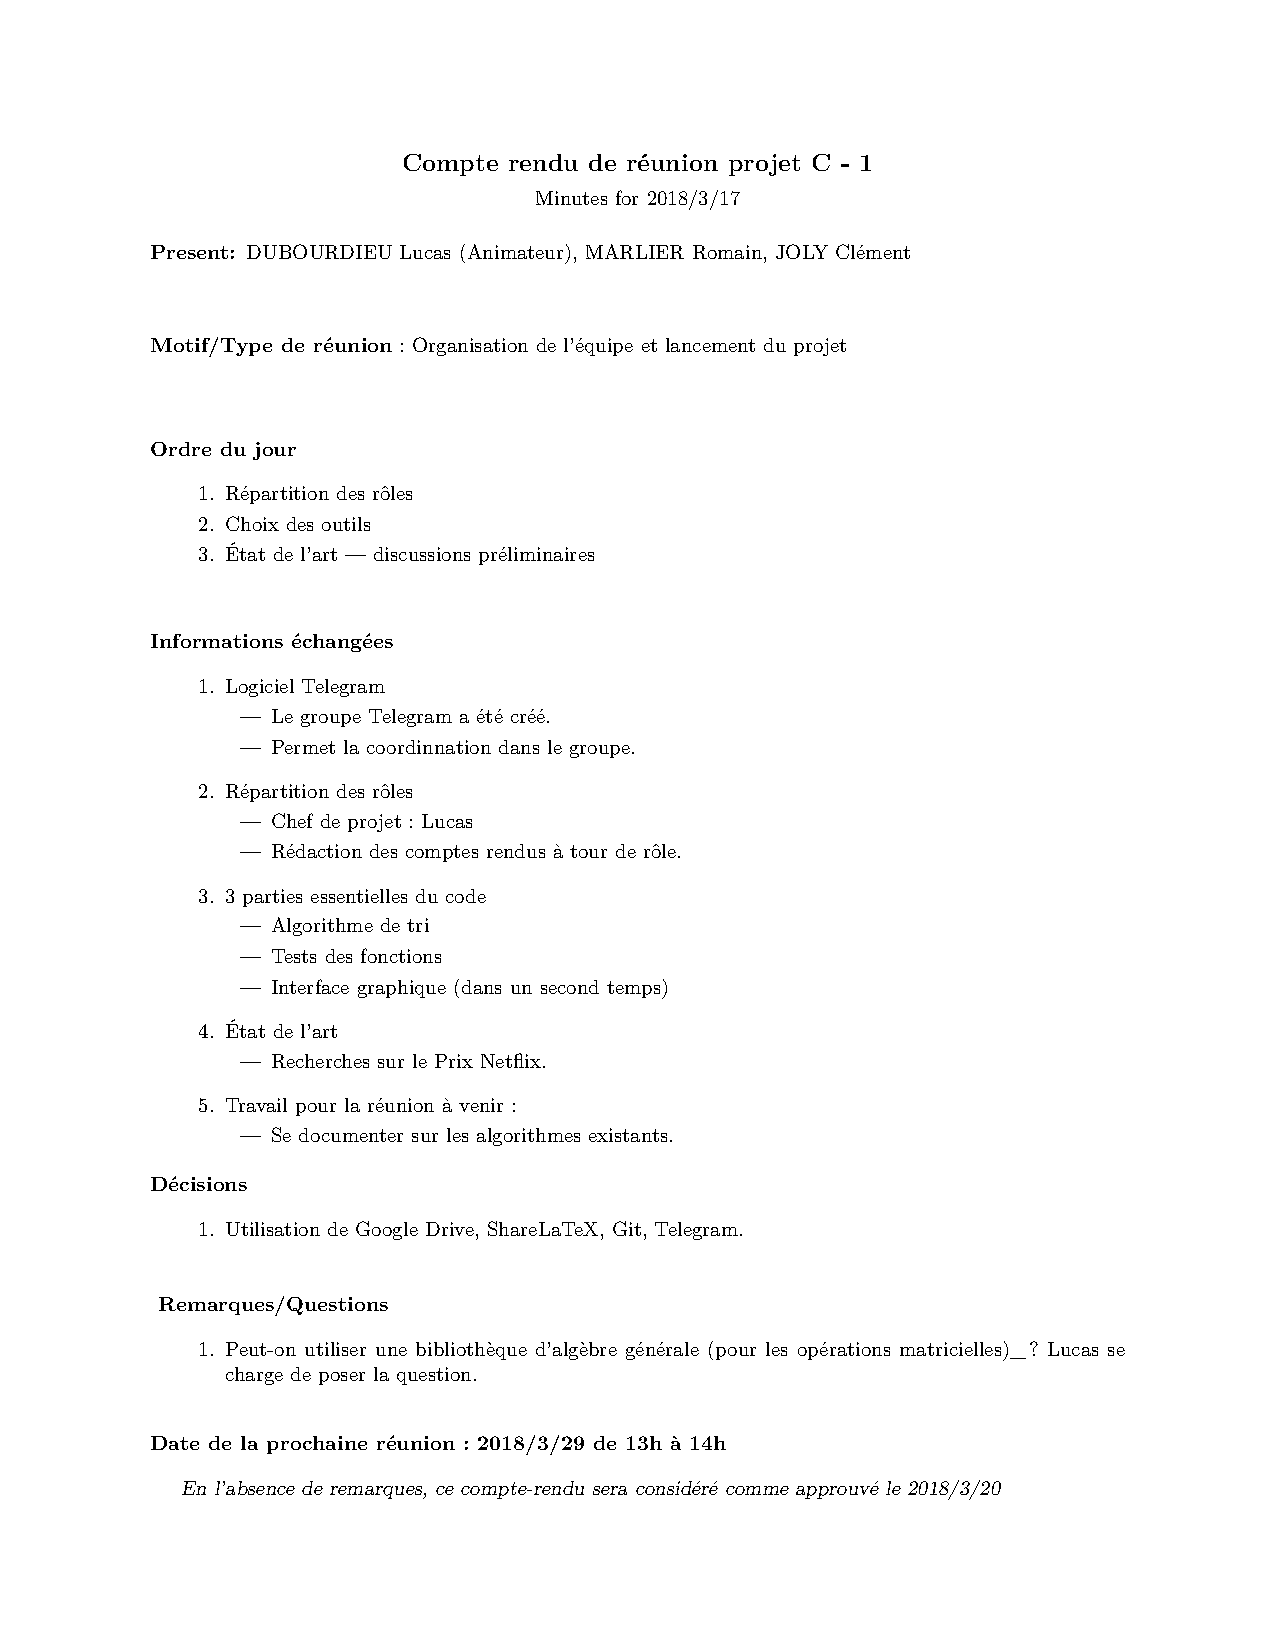
\includepdf[pages={1}]{CR/1.pdf}
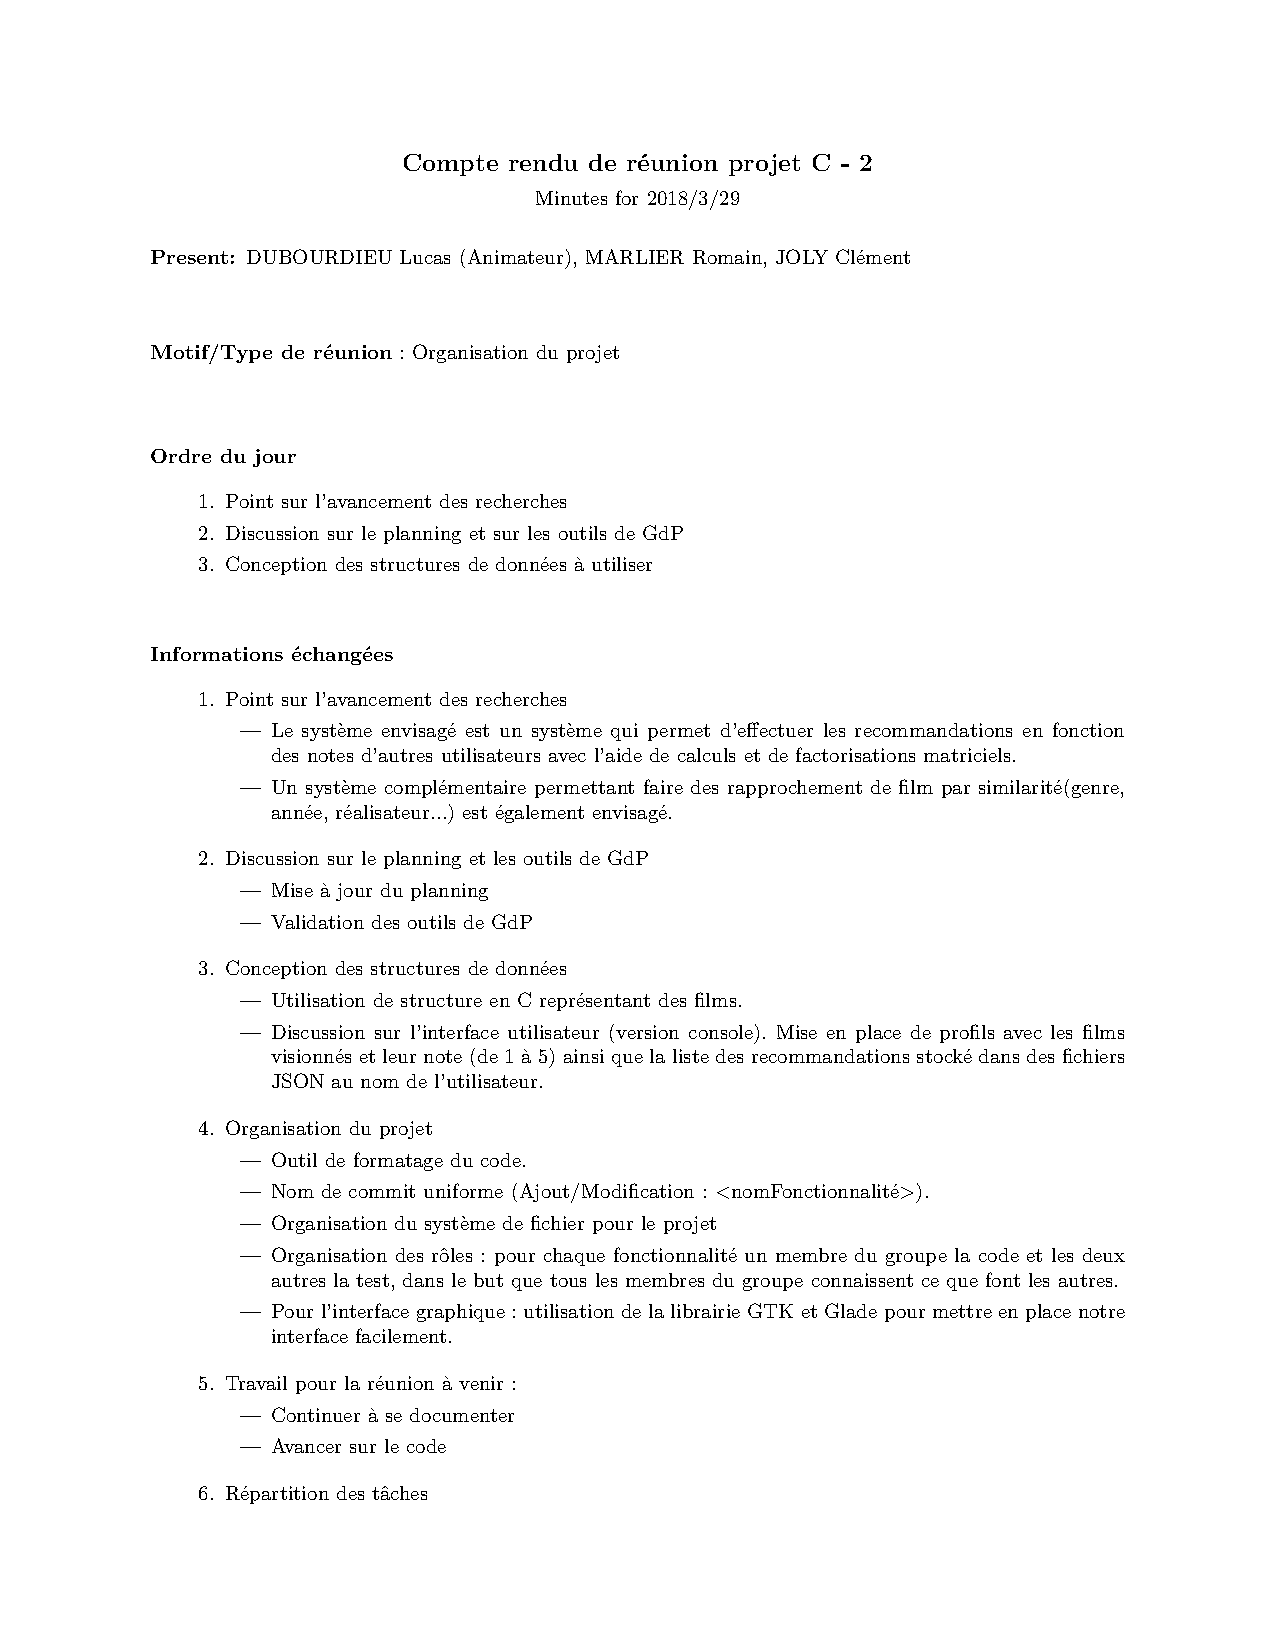
\includepdf[pages={1-2}]{CR/2.pdf}
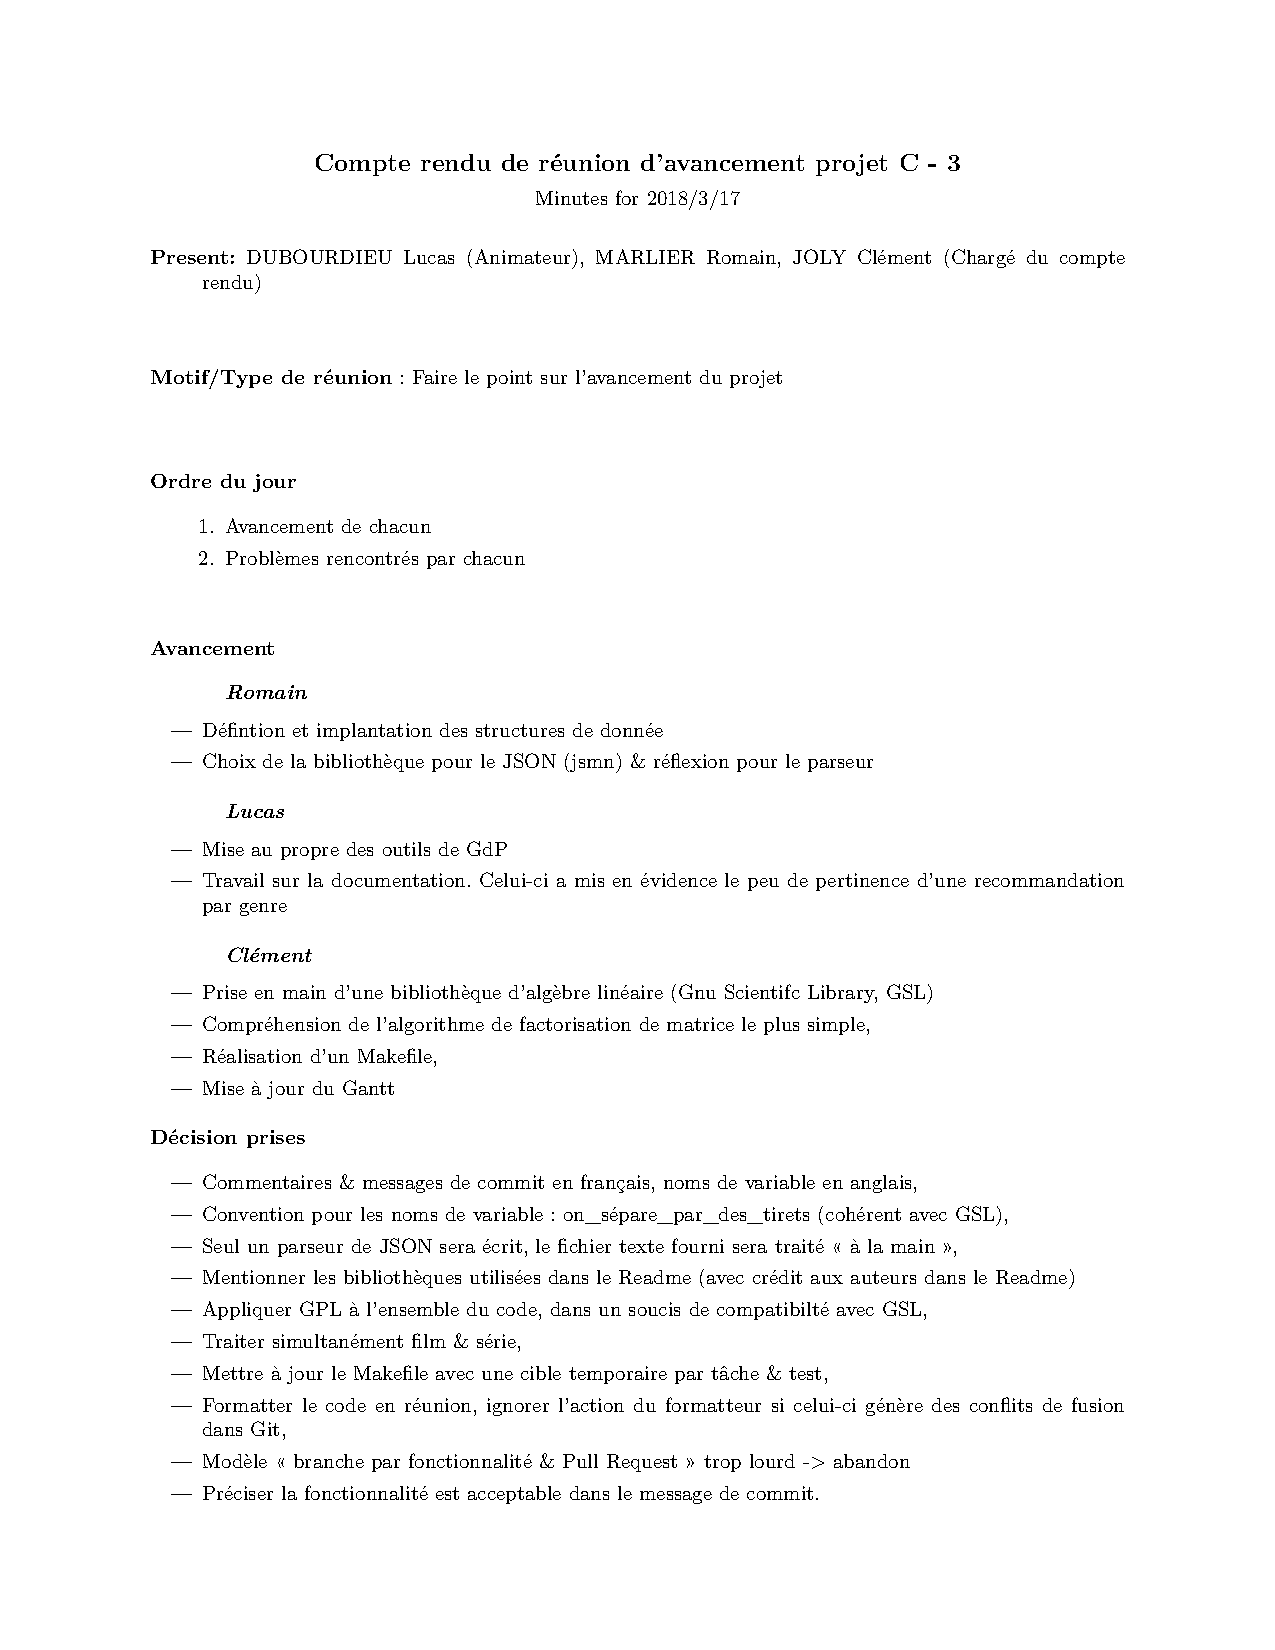
\includepdf[pages={1-2}]{CR/3.pdf}
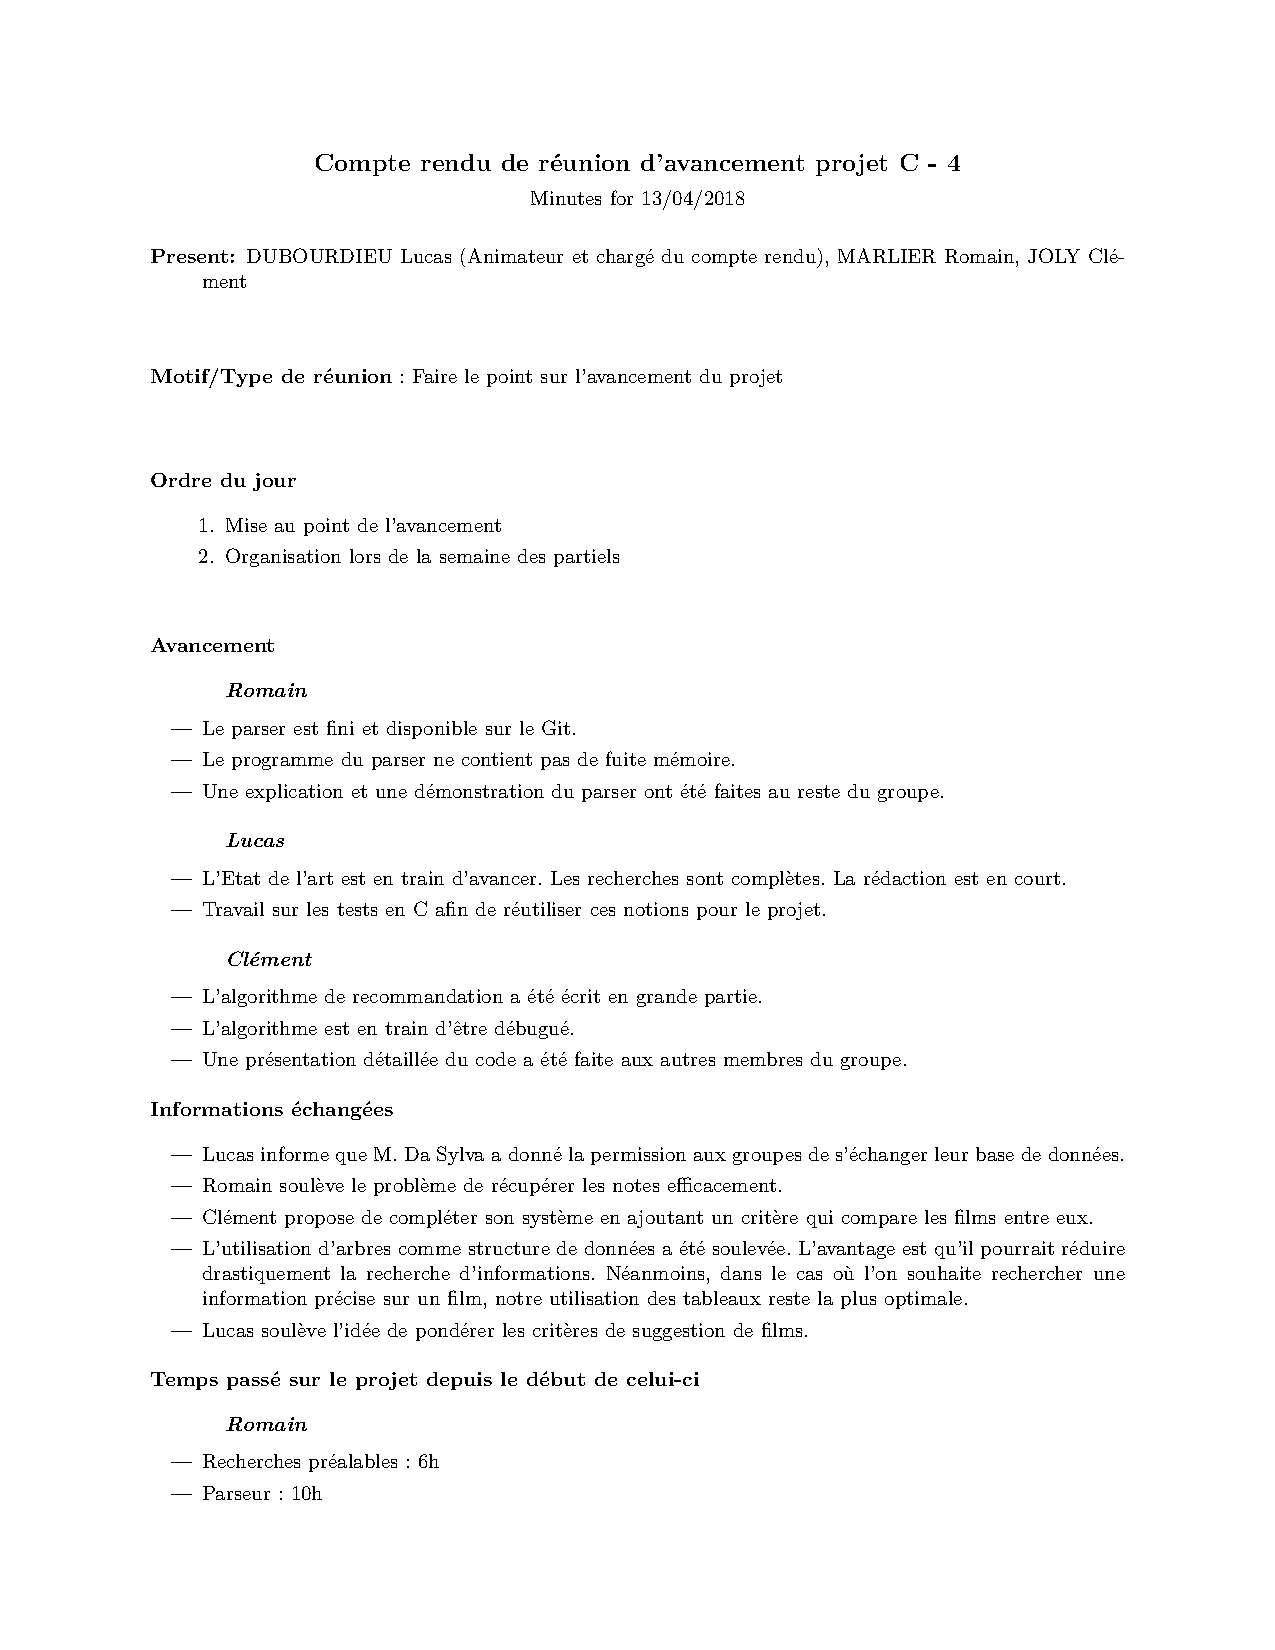
\includepdf[pages={1-2}]{CR/4.pdf}
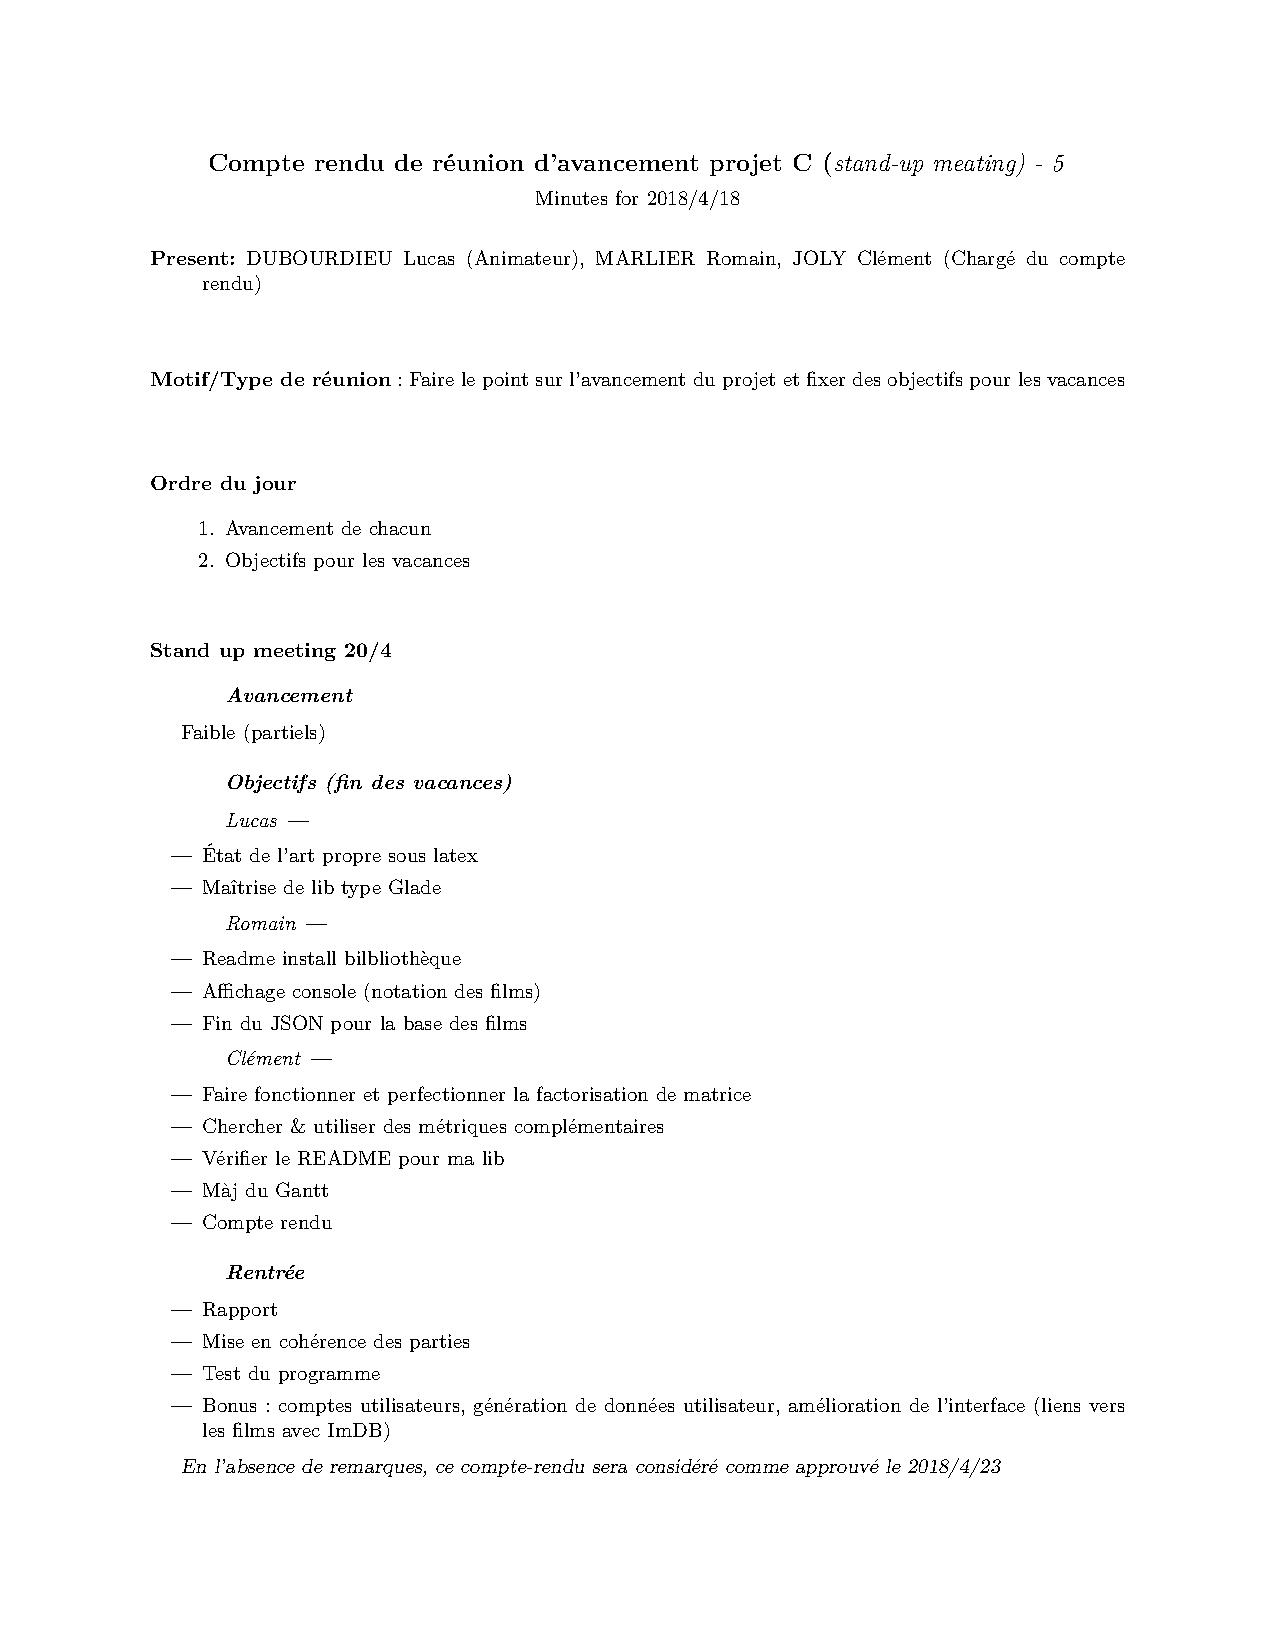
\includepdf[pages={1}]{CR/5.pdf}
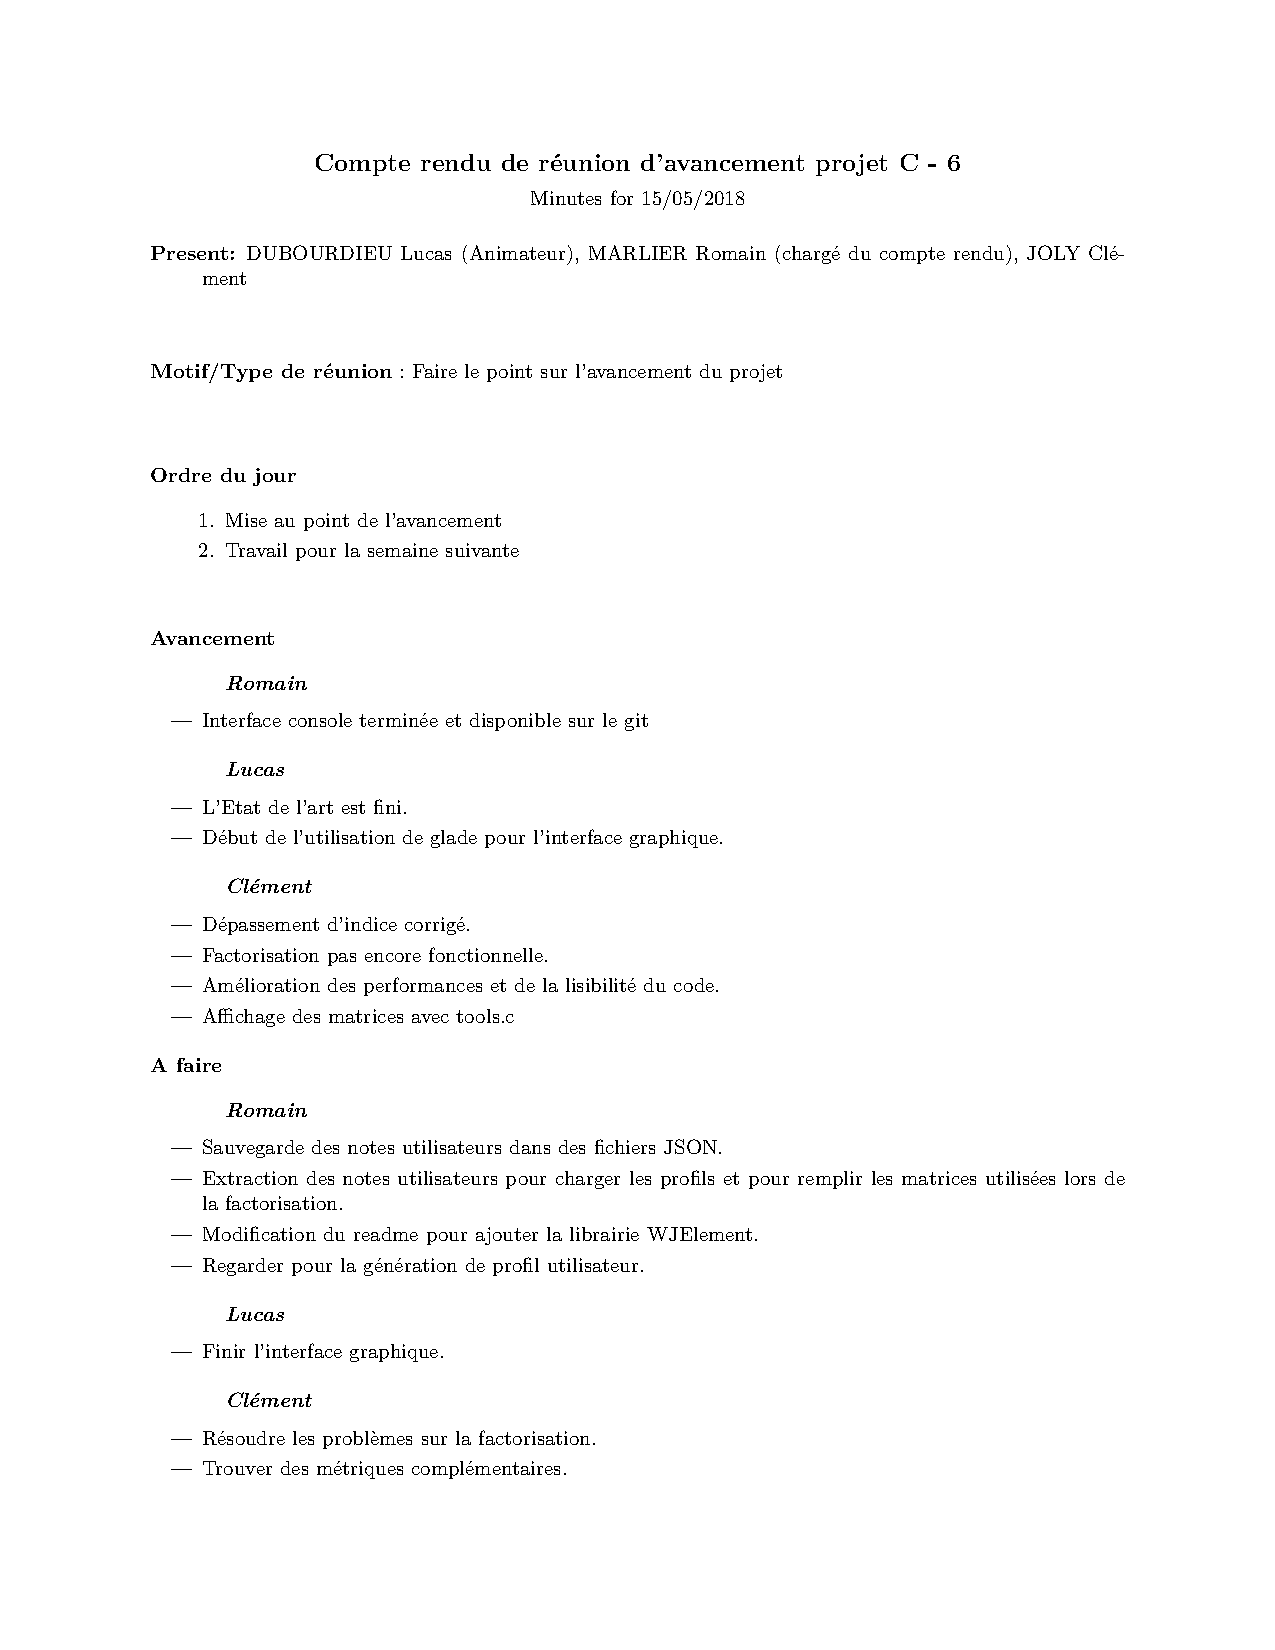
\includepdf[pages={1-2}]{CR/6.pdf}
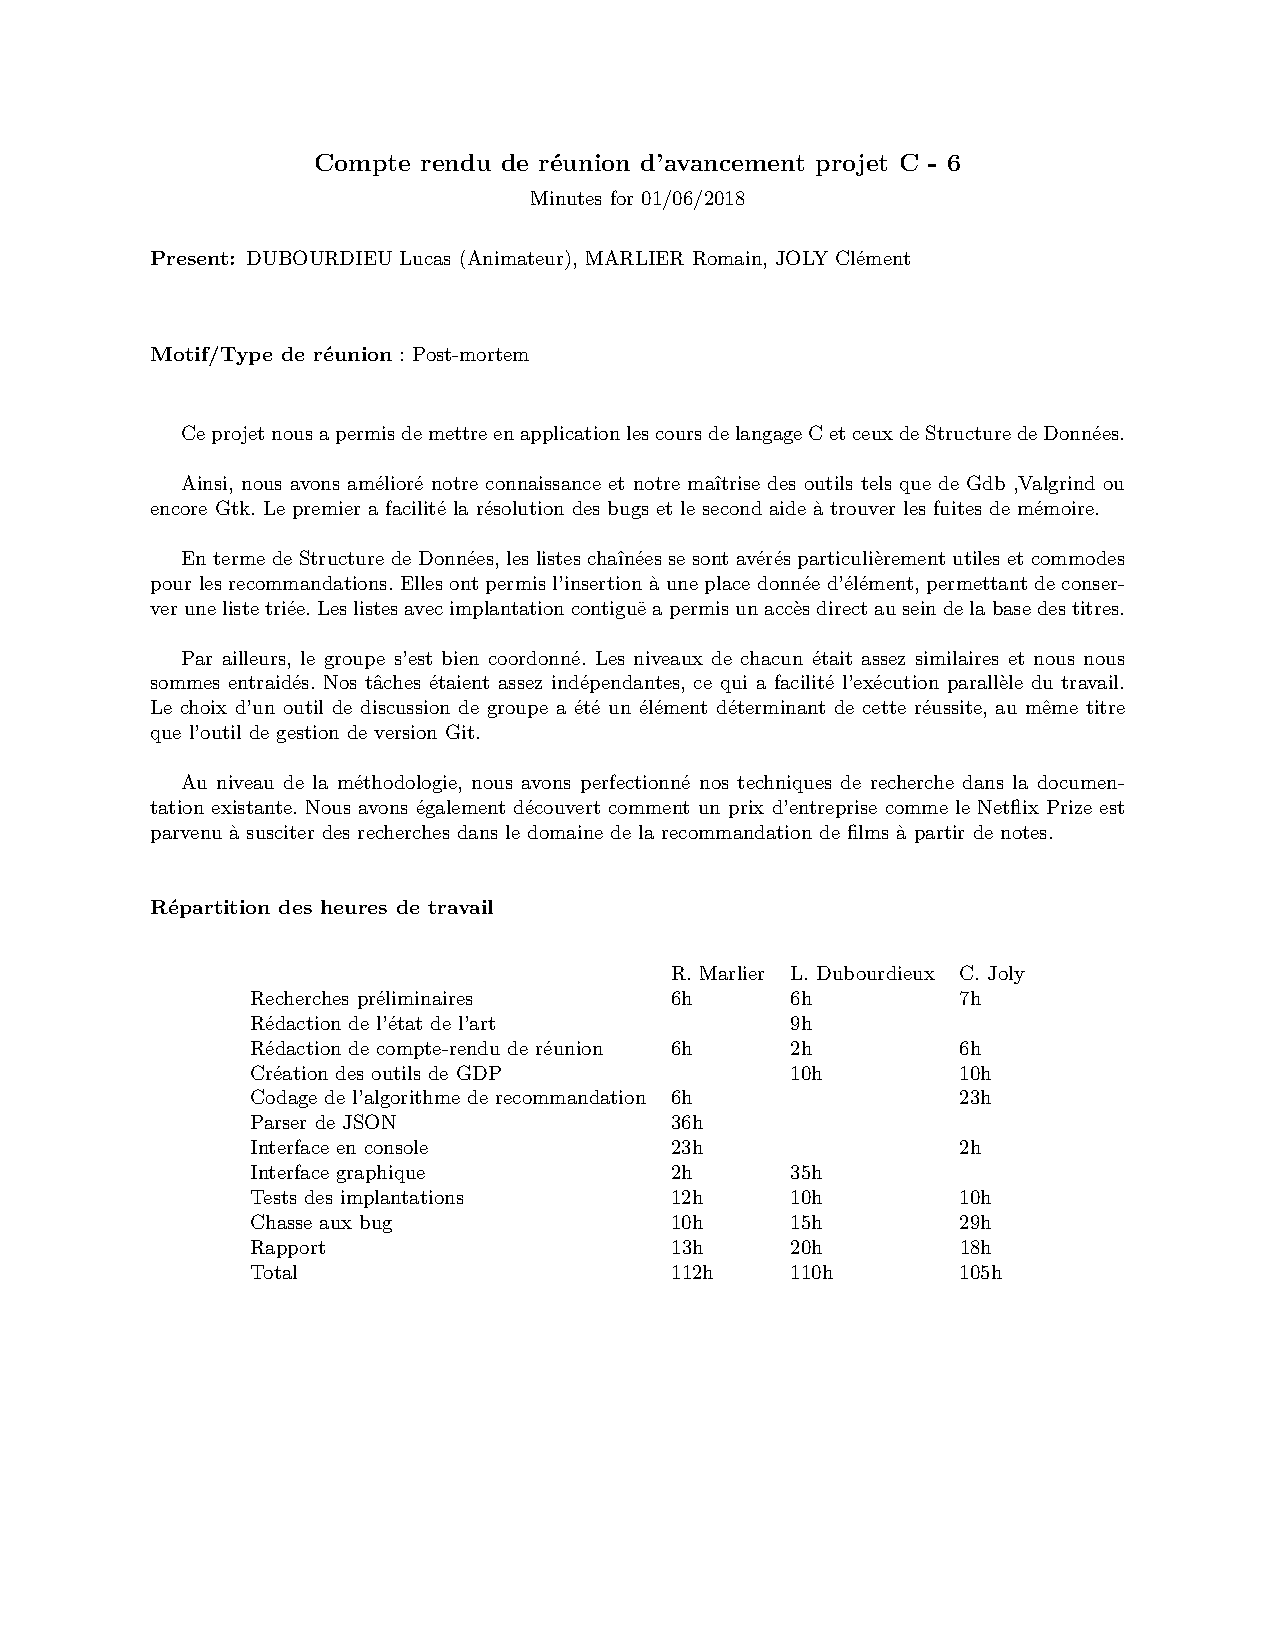
\includepdf[pages={1}]{CR/postmortem.pdf}

\subsection*{Sources}
\addcontentsline{toc}{subsection}{Sources}
\textbf{MOOC :} \\
https://gestiondeprojet.pm

\end{document}
